\chapter{Asynchronous Programming}\label{async}

\epigraphhead[30]{
\epigraph{\hspace*{-.1cm}\itshape``Who can wait quietly while the mud settles?\break
Who can remain still until the moment of action?''}%
{---Laozi, Tao Te Ching}
}\index{Laozi}

The central part of a computer, the part that carries out the individual steps that make up our programs, is called the \emph{\index{processor}processor}. The programs we have seen so far are things that will keep the processor busy until they have finished their work. The speed at which something like a loop that manipulates numbers can be executed depends pretty much entirely on the speed of the processor.\index{memory!speed}\index{network!speed}

But many programs interact with things outside of the processor. For example, they may communicate over a computer network or request data from the \index{hard disk}hard disk—which is a lot slower than getting it from memory.

When such a thing is happening, it would be a shame to let the processor sit idle—there might be some other work it could do in the meantime. In part, this is handled by your operating system, which will switch the processor between multiple running programs. But that doesn't help when we want a \emph{single} program to be able to make progress while it is waiting for a network request.

\section{Asynchronicity}\index{synchronous programming}

In a \emph{synchronous} programming model, things happen one at a time. When you call a function that performs a long-running action, it returns only when the action has finished and it can return the result. This stops your program for the time the action takes.\index{asynchronous programming}

An \emph{asynchronous} model allows multiple things to happen at the same time. When you start an action, your program continues to run. When the action finishes, the program is informed and gets access to the result (for example, the data read from disk).

We can compare synchronous and asynchronous programming using a small example: a program that fetches two resources from the \index{network}network and then combines results.\index{synchronous programming}

In a synchronous environment, where the request function returns only after it has done its work, the easiest way to perform this task is to make the requests one after the other. This has the drawback that the second request will be started only when the first has finished. The total time taken will be at least the sum of the two response times.\index{parallelism}

The solution to this problem, in a synchronous system, is to start additional \index{thread}threads of control. A \emph{thread} is another running program whose execution may be interleaved with other programs by the operating system—since most modern computers contain multiple processors, multiple threads may even run at the same time, on different processors. A second thread could start the second request, and then both threads wait for their results to come back, after which they resynchronize to combine their results.\index{CPU}\index{blocking}\index{asynchronous programming}\index{timeline}\index{callback function}

In the following diagram, the thick lines represent time the program spends running normally, and the thin lines represent time spent waiting for the network. In the synchronous model, the time taken by the network is \emph{part} of the timeline for a given thread of control. In the asynchronous model, starting a network action conceptually causes a \emph{split} in the timeline. The program that initiated the action continues running, and the action happens alongside it, notifying the program when it is finished.

\vskip 1.5ex
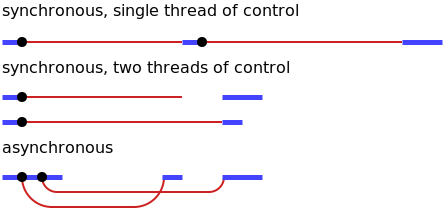
\includegraphics[width=8cm]{img/generated/control-io.pdf}
\vskip 1.5ex\index{control flow!asynchronous}\index{asynchronous programming}\index{verbosity}

Another way to describe the difference is that waiting for actions to finish is \emph{implicit} in the synchronous model, while it is \emph{explicit}, under our control, in the asynchronous one.

Asynchronicity cuts both ways. It makes expressing programs that do not fit the straight-line model of control easier, but it can also make expressing programs that do follow a straight line more awkward. We'll see some ways to address this awkwardness later in the chapter.

Both of the important JavaScript programming platforms—\index{browser}browsers and \index{Node.js}Node.js—make operations that might take a while asynchronous, rather than relying on \index{thread}threads. Since programming with threads is notoriously hard (understanding what a program does is much more difficult when it's doing multiple things at once), this is generally considered a good thing.

\section{Crow tech}

Most people are aware of the fact that \index{crow}crows are very smart birds. They can use tools, plan ahead, remember things, and even communicate these things among themselves.

What most people don't know is that they are capable of many things that they keep well hidden from us. I've been told by a reputable (if somewhat eccentric) expert on \index{corvid}corvids that crow technology is not far behind human technology, and they are catching up.

For example, many crow cultures have the ability to construct computing devices. These are not electronic, as human computing devices are, but operate through the actions of tiny insects, a species closely related to the \index{termite}termite, which has developed a \index{symbiotic relationship}symbiotic relationship with the crows. The birds provide them with food, and in return the insects build and operate their complex colonies that, with the help of the living creatures inside them, perform computations.

Such colonies are usually located in big, long-lived nests. The birds and insects work together to build a network of bulbous clay structures, hidden between the twigs of the nest, in which the insects live and work.

To communicate with other devices, these machines use light signals. The crows embed pieces of reflective material in special communication stalks, and the insects aim these to reflect light at another nest, encoding data as a sequence of quick flashes. This means that only nests that have an unbroken visual connection can communicate.

Our friend the corvid expert has mapped the network of crow nests in the village of \index{Hières-sur-Amby}Hières-sur-Amby, on the banks of the river Rhône. This map shows the nests and their connections:

\vskip 1.5ex
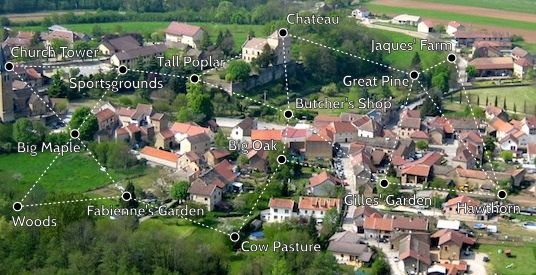
\includegraphics[width=10cm]{img/Hieres-sur-Amby.png}
\vskip 1.5ex

In an astounding example of \index{convergent evolution}convergent evolution, crow computers run JavaScript. In this chapter we'll write some basic networking functions for them.

\section{Callbacks}\index{function!callback|see{callback function}}

One approach to \index{asynchronous programming}asynchronous programming is to make functions that perform a slow action take an extra argument, a \emph{\index{callback
function}callback
function}. The action is started, and when it finishes, the callback function is called with the result.\index{setTimeout function}\index{waiting}

As an example, the \lstinline`setTimeout` function, available both in Node.js and in browsers, waits a given number of milliseconds (a second is a thousand milliseconds) and then calls a function.

\begin{lstlisting}
setTimeout(() => console.log("Tick"), 500);
\end{lstlisting}
\noindent

Waiting is not generally a very important type of work, but it can be useful when doing something like updating an animation or checking whether something is taking longer than a given amount of \index{time}time.

Performing multiple asynchronous actions in a row using callbacks means that you have to keep passing new functions to handle the \index{continuation}continuation of the computation after the actions.\index{hard disk}

Most crow nest computers have a long-term data storage bulb, where pieces of information are etched into twigs so that they can be retrieved later. Etching, or finding a piece of data, takes a moment, so the interface to long-term storage is asynchronous and uses callback functions.

Storage bulbs store pieces of \index{JSON}JSON-encodable data under names. A \index{crow}crow might store information about the places where it's hidden food under the name \lstinline`"food caches"`, which could hold an array of names that point at other pieces of data, describing the actual cache. To look up a food \index{cache}cache in the storage bulbs of the \emph{Big Oak} nest, a crow could run code like this:\index{readStorage function}

\begin{lstlisting}
import {bigOak} from "./crow-tech";

bigOak.readStorage("food caches", caches => {
  let firstCache = caches[0];
  bigOak.readStorage(firstCache, info => {
    console.log(info);
  });
});
\end{lstlisting}
\noindent

(All binding names and strings have been translated from crow language to English.)

This style of programming is workable, but the indentation level increases with each asynchronous action because you end up in another function. Doing more complicated things, such as running multiple actions at the same time, can get a little awkward.

Crow nest computers are built to communicate using \index{request}request-\index{response}response pairs. That means one nest sends a message to another nest, which then immediately sends a message back, confirming receipt and possibly including a reply to a question asked in the message.

Each message is tagged with a \emph{type}, which determines how it is handled. Our code can define handlers for specific request types, and when such a request comes in, the handler is called to produce a response.\index{crow-tech module}\index{send method}

The interface exported by the \lstinline`"./crow-tech"` module provides callback-based functions for communication. Nests have a \lstinline`send` method that sends off a request. It expects the name of the target nest, the type of the request, and the content of the request as its first three arguments, and it expects a function to call when a response comes in as its fourth and last argument.

\begin{lstlisting}
bigOak.send("Cow Pasture", "note", "Let's caw loudly at 7PM",
            () => console.log("Note delivered."));
\end{lstlisting}
\noindent

But to make nests capable of receiving that request, we first have to define a \index{request type}request type named \lstinline`"note"`. The code that handles the requests has to run not just on this nest-computer but on all nests that can receive messages of this type. We'll just assume that a crow flies over and installs our handler code on all the nests.\index{defineRequestType function}

\begin{lstlisting}
import {defineRequestType} from "./crow-tech";

defineRequestType("note", (nest, content, source, done) => {
  console.log(`${nest.name} received note: ${content}`);
  done();
});
\end{lstlisting}
\noindent

The \lstinline`defineRequestType` function defines a new type of request. The example adds support for \lstinline`"note"` requests, which just sends a note to a given nest. Our implementation calls \lstinline`console.log` so that we can verify that the request arrived. Nests have a \lstinline`name` property that holds their name.\index{asynchronous programming}

The fourth argument given to the handler, \lstinline`done`, is a callback function that it must call when it is done with the request. If we had used the handler's \index{return value}return value as the response value, that would mean that a request handler can't itself perform asynchronous actions. A function doing asynchronous work typically returns before the work is done, having arranged for a callback to be called when it completes. So we need some asynchronous mechanism—in this case, another \index{callback function}callback function—to signal when a response is available.

In a way, asynchronicity is \emph{contagious}. Any function that calls a function that works asynchronously must itself be asynchronous, using a callback or similar mechanism to deliver its result. Calling a callback is somewhat more involved and error-prone than simply returning a value, so needing to structure large parts of your program that way is not great.

\section{Promises}

Working with abstract concepts is often easier when those concepts can be represented by \index{value}values. In the case of asynchronous actions, you could, instead of arranging for a function to be called at some point in the future, return an object that represents this future event.\index{Promise class}\index{asynchronous programming}

This is what the standard class \lstinline`Promise` is for. A \emph{promise} is an asynchronous action that may complete at some point and produce a value. It is able to notify anyone who is interested when its value is available.\index{Promise.resolve function}\index{resolving (a promise)}

The easiest way to create a promise is by calling \lstinline`Promise.resolve`. This function ensures that the value you give it is wrapped in a promise. If it's already a promise, it is simply returned—otherwise, you get a new promise that immediately finishes with your value as its result.

\begin{lstlisting}
let fifteen = Promise.resolve(15);
fifteen.then(value => console.log(`Got ${value}`));
// → Got 15
\end{lstlisting}
\noindent\index{then method}

To get the result of a promise, you can use its \lstinline`then` method. This registers a \index{callback function}callback function to be called when the promise resolves and produces a value. You can add multiple callbacks to a single promise, and they will be called, even if you add them after the promise has already \emph{resolved} (finished).

But that's not all the \lstinline`then` method does. It returns another promise, which resolves to the value that the handler function returns or, if that returns a promise, waits for that promise and then resolves to its result.

It is useful to think of promises as a device to move values into an asynchronous reality. A normal value is simply there. A promised value is a value that \emph{might} already be there or might appear at some point in the future. Computations defined in terms of promises act on such wrapped values and are executed asynchronously as the values become available.\index{Promise class}

To create a promise, you can use \lstinline`Promise` as a constructor. It has a somewhat odd interface—the constructor expects a function as argument, which it immediately calls, passing it a function that it can use to resolve the promise. It works this way, instead of for example with a \lstinline`resolve` method, so that only the code that created the promise can resolve it.\index{storage function}

This is how you'd create a promise-based interface for the \lstinline`readStorage` function:

\begin{lstlisting}
function storage(nest, name) {
  return new Promise(resolve => {
    nest.readStorage(name, result => resolve(result));
  });
}

storage(bigOak, "enemies")
  .then(value => console.log("Got", value));
\end{lstlisting}
\noindent

This asynchronous function returns a meaningful value. This is the main advantage of promises—they simplify the use of asynchronous functions. Instead of having to pass around callbacks, promise-based functions look similar to regular ones: they take input as arguments and return their output. The only difference is that the output may not be available yet.

\section{Failure}\index{exception handling}

Regular JavaScript computations can fail by throwing an exception. Asynchronous computations often need something like that. A network request may fail, or some code that is part of the asynchronous computation may throw an exception.\index{callback function}\index{error}

One of the most pressing problems with the callback style of asynchronous programming is that it makes it extremely difficult to make sure failures are properly reported to the callbacks.

A widely used convention is that the first argument to the callback is used to indicate that the action failed, and the second contains the value produced by the action when it was successful. Such callback functions must always check whether they received an exception and make sure that any problems they cause, including exceptions thrown by functions they call, are caught and given to the right function.\index{rejecting (a promise)}\index{resolving (a promise)}\index{then method}

Promises make this easier. They can be either resolved (the action finished successfully) or rejected (it failed). Resolve handlers (as registered with \lstinline`then`) are called only when the action is successful, and rejections are automatically propagated to the new promise that is returned by \lstinline`then`. And when a handler throws an exception, this automatically causes the promise produced by its \lstinline`then` call to be rejected. So if any element in a chain of asynchronous actions fails, the outcome of the whole chain is marked as rejected, and no success handlers are called beyond the point where it failed.\index{Promise.reject function}\index{Promise class}

Much like resolving a promise provides a value, rejecting one also provides one, usually called the \emph{reason} of the rejection. When an exception in a handler function causes the rejection, the exception value is used as the reason. Similarly, when a handler returns a promise that is rejected, that rejection flows into the next promise. There's a \lstinline`Promise.reject` function that creates a new, immediately rejected promise.\index{catch method}

To explicitly handle such rejections, promises have a \lstinline`catch` method that registers a handler to be called when the promise is rejected, similar to how \lstinline`then` handlers handle normal resolution. It's also very much like \lstinline`then` in that it returns a new promise, which resolves to the original promise's value if it resolves normally and to the result of the \lstinline`catch` handler otherwise. If a \lstinline`catch` handler throws an error, the new promise is also rejected.\index{then method}

As a shorthand, \lstinline`then` also accepts a rejection handler as a second argument, so you can install both types of handlers in a single method call.

A function passed to the \lstinline`Promise` constructor receives a second argument, alongside the resolve function, which it can use to reject the new promise.

The chains of promise values created by calls to \lstinline`then` and \lstinline`catch` can be seen as a pipeline through which asynchronous values or failures move. Since such chains are created by registering handlers, each link has a success handler or a rejection handler (or both) associated with it. Handlers that don't match the type of outcome (success or failure) are ignored. But those that do match are called, and their outcome determines what kind of value comes next—success when it returns a non-promise value, rejection when it throws an exception, and the outcome of a promise when it returns one of those.

\begin{lstlisting}
new Promise((_, reject) => reject(new Error("Fail")))
  .then(value => console.log("Handler 1"))
  .catch(reason => {
    console.log("Caught failure " + reason);
    return "nothing";
  })
  .then(value => console.log("Handler 2", value));
// → Caught failure Error: Fail
// → Handler 2 nothing
\end{lstlisting}
\noindent\index{uncaught exception}\index{exception handling}

Much like an uncaught exception is handled by the environment, JavaScript environments can detect when a promise rejection isn't handled and will report this as an error.

\section{Networks are hard}\index{network!reliability}

Occasionally, there isn't enough light for the \index{crow}crows' mirror systems to transmit a signal or something is blocking the path of the signal. It is possible for a signal to be sent but never received.\index{send method}\index{error}\index{timeout}

As it is, that will just cause the callback given to \lstinline`send` to never be called, which will probably cause the program to stop without even noticing there is a problem. It would be nice if, after a given period of not getting a response, a request would \emph{time out} and report failure.

Often, transmission failures are random accidents, like a car's headlight interfering with the light signals, and simply retrying the request may cause it to succeed. So while we're at it, let's make our request function automatically retry the sending of the request a few times before it gives up.\index{Promise class}\index{callback function}\index{interface!object}

And, since we've established that promises are a good thing, we'll also make our request function return a promise. In terms of what they can express, callbacks and promises are equivalent. Callback-based functions can be wrapped to expose a promise-based interface, and vice versa.

Even when a \index{request}request and its \index{response}response are successfully delivered, the response may indicate failure—for example, if the request tries to use a request type that hasn't been defined or the handler throws an error. To support this, \lstinline`send` and \lstinline`defineRequestType` follow the convention mentioned before, where the first argument passed to callbacks is the failure reason, if any, and the second is the actual result.

These can be translated to promise resolution and rejection by our wrapper.\index{Timeout class}\index{request function}\index{retry}

\begin{lstlisting}
class Timeout extends Error {}

function request(nest, target, type, content) {
  return new Promise((resolve, reject) => {
    let done = false;
    function attempt(n) {
      nest.send(target, type, content, (failed, value) => {
        done = true;
        if (failed) reject(failed);
        else resolve(value);
      });
      setTimeout(() => {
        if (done) return;
        else if (n < 3) attempt(n + 1);
        else reject(new Timeout("Timed out"));
      }, 250);
    }
    attempt(1);
  });
}
\end{lstlisting}
\noindent\index{Promise class}\index{resolving (a promise)}\index{rejecting (a promise)}

Because promises can be resolved (or rejected) only once, this will work. The first time \lstinline`resolve` or \lstinline`reject` is called determines the outcome of the promise, and any further calls, such as the timeout arriving after the request finishes or a request coming back after another request finished, are ignored.\index{recursion}

To build an asynchronous \index{loop}loop, for the retries, we need to use a recursive function—a regular loop doesn't allow us to stop and wait for an asynchronous action. The \lstinline`attempt` function makes a single attempt to send a request. It also sets a timeout that, if no response has come back after 250 milliseconds, either starts the next attempt or, if this was the fourth attempt, rejects the promise with an instance of \lstinline`Timeout` as the reason.\index{idempotence}

Retrying every quarter-second and giving up when no response has come in after a second is definitely somewhat arbitrary. It is even possible, if the request did come through but the handler is just taking a bit longer, for requests to be delivered multiple times. We'll write our handlers with that problem in mind—duplicate messages should be harmless.

In general, we will not be building a world-class, robust network today. But that's okay—crows don't have very high expectations yet when it comes to computing.\index{defineRequestType function}\index{requestType function}

To isolate ourselves from callbacks altogether, we'll go ahead and also define a wrapper for \lstinline`defineRequestType` that allows the handler function to return a promise or plain value and wires that up to the callback for us.

\begin{lstlisting}
function requestType(name, handler) {
  defineRequestType(name, (nest, content, source,
                           callback) => {
    try {
      Promise.resolve(handler(nest, content, source))
        .then(response => callback(null, response),
              failure => callback(failure));
    } catch (exception) {
      callback(exception);
    }
  });
}
\end{lstlisting}
\noindent\index{Promise.resolve function}

\lstinline`Promise.resolve` is used to convert the value returned by \lstinline`handler` to a promise if it isn't already.\index{try keyword}\index{callback function}

Note that the call to \lstinline`handler` had to be wrapped in a \lstinline`try` block to make sure any exception it raises directly is given to the callback. This nicely illustrates the difficulty of properly handling errors with raw callbacks—it is easy to forget to properly route exceptions like that, and if you don't do it, failures won't get reported to the right callback. Promises make this mostly automatic and thus less error-prone.

\section{Collections of promises}\index{neighbors property}\index{ping request}

Each nest computer keeps an array of other nests within transmission distance in its \lstinline`neighbors` property. To check which of those are currently reachable, you could write a function that tries to send a \lstinline`"ping"` request (a request that simply asks for a response) to each of them and see which ones come back.\index{Promise.all function}

When working with collections of promises running at the same time, the \lstinline`Promise.all` function can be useful. It returns a promise that waits for all of the promises in the array to resolve and then resolves to an array of the values that these promises produced (in the same order as the original array). If any promise is rejected, the result of \lstinline`Promise.all` is itself rejected.

\begin{lstlisting}
requestType("ping", () => "pong");

function availableNeighbors(nest) {
  let requests = nest.neighbors.map(neighbor => {
    return request(nest, neighbor, "ping")
      .then(() => true, () => false);
  });
  return Promise.all(requests).then(result => {
    return nest.neighbors.filter((_, i) => result[i]);
  });
}
\end{lstlisting}
\noindent\index{then method}

When a neighbor isn't available, we don't want the entire combined promise to fail since then we still wouldn't know anything. So the function that is mapped over the set of neighbors to turn them into request promises attaches handlers that make successful requests produce \lstinline`true` and rejected ones produce \lstinline`false`.\index{filter method}\index{map method}\index{some method}

In the handler for the combined promise, \lstinline`filter` is used to remove those elements from the \lstinline`neighbors` array whose corresponding value is false. This makes use of the fact that \lstinline`filter` passes the array index of the current element as a second argument to its filtering function (\lstinline`map`, \lstinline`some`, and similar higher-order array methods do the same).

\section{Network flooding}

The fact that nests can talk only to their neighbors greatly inhibits the usefulness of this network.

For broadcasting information to the whole network, one solution is to set up a type of request that is automatically forwarded to neighbors. These neighbors then in turn forward it to their neighbors, until the whole network has received the message.\index{sendGossip function}

\begin{lstlisting}
import {everywhere} from "./crow-tech";

everywhere(nest => {
  nest.state.gossip = [];
});

function sendGossip(nest, message, exceptFor = null) {
  nest.state.gossip.push(message);
  for (let neighbor of nest.neighbors) {
    if (neighbor == exceptFor) continue;
    request(nest, neighbor, "gossip", message);
  }
}

requestType("gossip", (nest, message, source) => {
  if (nest.state.gossip.includes(message)) return;
  console.log(`${nest.name} received gossip '${
               message}' from ${source}`);
  sendGossip(nest, message, source);
});
\end{lstlisting}
\noindent\index{everywhere function}\index{gossip property}

To avoid sending the same message around the network forever, each nest keeps an array of gossip strings that it has already seen. To define this array, we use the \lstinline`everywhere` function—which runs code on every nest—to add a property to the nest's \lstinline`state` object, which is where we'll keep nest-local state.

When a nest receives a duplicate gossip message, which is very likely to happen with everybody blindly resending them, it ignores it. But when it receives a new message, it excitedly tells all its neighbors except for the one who sent it the message.

This will cause a new piece of gossip to spread through the network like an ink stain in water. Even when some connections aren't currently working, if there is an alternative route to a given nest, the gossip will reach it through there.\index{flooding}

This style of network communication is called \emph{flooding}—it floods the network with a piece of information until all nodes have it.

\section{Message routing}\index{efficiency}

If a given node wants to talk to a single other node, flooding is not a very efficient approach. Especially when the network is big, that would lead to a lot of useless data transfers.\index{routing}

An alternative approach is to set up a way for messages to hop from node to node until they reach their destination. The difficulty with that is it requires knowledge about the layout of the network. To send a request in the direction of a faraway nest, it is necessary to know which neighboring nest gets it closer to its destination. Sending it in the wrong direction will not do much good.

Since each nest knows only about its direct neighbors, it doesn't have the information it needs to compute a route. We must somehow spread the information about these connections to all nests, preferably in a way that allows it to change over time, when nests are abandoned or new nests are built.\index{flooding}

We can use flooding again, but instead of checking whether a given message has already been received, we now check whether the new set of neighbors for a given nest matches the current set we have for it.\index{broadcastConnections function}\index{connections binding}

\begin{lstlisting}
requestType("connections", (nest, {name, neighbors},
                            source) => {
  let connections = nest.state.connections;
  if (JSON.stringify(connections.get(name)) ==
      JSON.stringify(neighbors)) return;
  connections.set(name, neighbors);
  broadcastConnections(nest, name, source);
});

function broadcastConnections(nest, name, exceptFor = null) {
  for (let neighbor of nest.neighbors) {
    if (neighbor == exceptFor) continue;
    request(nest, neighbor, "connections", {
      name,
      neighbors: nest.state.connections.get(name)
    });
  }
}

everywhere(nest => {
  nest.state.connections = new Map;
  nest.state.connections.set(nest.name, nest.neighbors);
  broadcastConnections(nest, nest.name);
});
\end{lstlisting}
\noindent\index{JSON}\index{== operator}

The comparison uses \lstinline`JSON.stringify` because \lstinline`==`, on objects or arrays, will return true only when the two are the exact same value, which is not what we need here. Comparing the JSON strings is a crude but effective way to compare their content.

The nodes immediately start broadcasting their connections, which should, unless some nests are completely unreachable, quickly give every nest a map of the current network \index{graph}graph.\index{pathfinding}

A thing you can do with graphs is find routes in them, as we saw in \hyperref[robot]{Chapter 7}. If we have a route toward a message's destination, we know which direction to send it in.\index{findRoute function}

This \lstinline`findRoute` function, which greatly resembles the \lstinline`findRoute` from \hyperref[robot.findRoute]{Chapter 7}, searches for a way to reach a given node in the network. But instead of returning the whole route, it just returns the next step. That next nest will itself, using its current information about the network, decide where \emph{it} sends the message.

\begin{lstlisting}
function findRoute(from, to, connections) {
  let work = [{at: from, via: null}];
  for (let i = 0; i < work.length; i++) {
    let {at, via} = work[i];
    for (let next of connections.get(at) || []) {
      if (next == to) return via;
      if (!work.some(w => w.at == next)) {
        work.push({at: next, via: via || next});
      }
    }
  }
  return null;
}
\end{lstlisting}
\noindent

Now we can build a function that can send long-distance messages. If the message is addressed to a direct neighbor, it is delivered as usual. If not, it is packaged in an object and sent to a neighbor that is closer to the target, using the \lstinline`"route"` request type, which will cause that neighbor to repeat the same behavior.\index{routeRequest function}

\begin{lstlisting}
function routeRequest(nest, target, type, content) {
  if (nest.neighbors.includes(target)) {
    return request(nest, target, type, content);
  } else {
    let via = findRoute(nest.name, target,
                        nest.state.connections);
    if (!via) throw new Error(`No route to ${target}`);
    return request(nest, via, "route",
                   {target, type, content});
  }
}

requestType("route", (nest, {target, type, content}) => {
  return routeRequest(nest, target, type, content);
});
\end{lstlisting}
\noindent\index{network!abstraction}\index{layering}

We've constructed several layers of functionality on top of a primitive communication system to make it convenient to use. This is a nice (though simplified) model of how real computer networks work.\index{error}

A distinguishing property of computer networks is that they aren't reliable—abstractions built on top of them can help, but you can't abstract away network failure. So network programming is typically very much about anticipating and dealing with failures.

\section{Async functions}

To store important information, \index{crow}crows are known to duplicate it across nests. That way, when a hawk destroys a nest, the information isn't lost.

To retrieve a given piece of information that it doesn't have in its own storage bulb, a nest computer might consult random other nests in the network until it finds one that has it.\index{findInStorage function}\index{network function}

\begin{lstlisting}
requestType("storage", (nest, name) => storage(nest, name));

function findInStorage(nest, name) {
  return storage(nest, name).then(found => {
    if (found != null) return found;
    else return findInRemoteStorage(nest, name);
  });
}

function network(nest) {
  return Array.from(nest.state.connections.keys());
}

function findInRemoteStorage(nest, name) {
  let sources = network(nest).filter(n => n != nest.name);
  function next() {
    if (sources.length == 0) {
      return Promise.reject(new Error("Not found"));
    } else {
      let source = sources[Math.floor(Math.random() *
                                      sources.length)];
      sources = sources.filter(n => n != source);
      return routeRequest(nest, source, "storage", name)
        .then(value => value != null ? value : next(),
              next);
    }
  }
  return next();
}
\end{lstlisting}
\noindent\index{Map class}\index{Object.keys function}\index{Array.from function}

Because \lstinline`connections` is a \lstinline`Map`, \lstinline`Object.keys` doesn't work on it. It has a \lstinline`keys` \emph{method}, but that returns an iterator rather than an array. An iterator (or iterable value) can be converted to an array with the \lstinline`Array.from` function.\index{Promise class}\index{recursion}

Even with promises this is some rather awkward code. Multiple asynchronous actions are chained together in non-obvious ways. We again need a recursive function (\lstinline`next`) to model looping through the nests.\index{synchronous programming}\index{asynchronous programming}

And the thing the code actually does is completely linear—it always waits for the previous action to complete before starting the next one. In a synchronous programming model, it'd be simpler to express.\index{async function}\index{await keyword}

The good news is that JavaScript allows you to write pseudo-synchronous code to describe asynchronous computation. An \lstinline`async` function is a function that implicitly returns a promise and that can, in its body, \lstinline`await` other promises in a way that \emph{looks} synchronous.\index{findInStorage function}

We can rewrite \lstinline`findInStorage` like this:

\begin{lstlisting}
async function findInStorage(nest, name) {
  let local = await storage(nest, name);
  if (local != null) return local;

  let sources = network(nest).filter(n => n != nest.name);
  while (sources.length > 0) {
    let source = sources[Math.floor(Math.random() *
                                    sources.length)];
    sources = sources.filter(n => n != source);
    try {
      let found = await routeRequest(nest, source, "storage",
                                     name);
      if (found != null) return found;
    } catch (_) {}
  }
  throw new Error("Not found");
}
\end{lstlisting}
\noindent\index{async function}\index{return keyword}\index{exception handling}

An \lstinline`async` function is marked by the word \lstinline`async` before the \lstinline`function` keyword. Methods can also be made \lstinline`async` by writing \lstinline`async` before their name. When such a function or method is called, it returns a promise. As soon as the body returns something, that promise is resolved. If it throws an exception, the promise is rejected.\index{await keyword}\index{control flow!asynchronous}

Inside an \lstinline`async` function, the word \lstinline`await` can be put in front of an expression to wait for a promise to resolve and only then continue the execution of the function.

Such a function no longer, like a regular JavaScript function, runs from start to completion in one go. Instead, it can be \emph{frozen} at any point that has an \lstinline`await`, and can be resumed at a later time.

For non-trivial asynchronous code, this notation is usually more convenient than directly using promises. Even if you need to do something that doesn't fit the synchronous model, such as perform multiple actions at the same time, it is easy to combine \lstinline`await` with the direct use of promises.

\section{Generators}\index{async function}

This ability of functions to be paused and then resumed again is not exclusive to \lstinline`async` functions. JavaScript also has a feature called \emph{\index{generator}generator} functions. These are similar, but without the promises.

When you define a function with \lstinline`function*` (placing an asterisk after the word \lstinline`function`), it becomes a generator. When you call a generator, it returns an \index{iterator}iterator, which we already saw in \hyperref[object]{Chapter 6}.

\begin{lstlisting}
function* powers(n) {
  for (let current = n;; current *= n) {
    yield current;
  }
}

for (let power of powers(3)) {
  if (power > 50) break;
  console.log(power);
}
// → 3
// → 9
// → 27
\end{lstlisting}
\noindent\index{next method}\index{yield keyword}

Initially, when you call \lstinline`powers`, the function is frozen at its start. Every time you call \lstinline`next` on the iterator, the function runs until it hits a \lstinline`yield` expression, which pauses it and causes the yielded value to become the next value produced by the iterator. When the function returns (the one in the example never does), the iterator is done.

Writing iterators is often much easier when you use generator functions. The iterator for the \lstinline`Group` class (from the exercise in \hyperref[object.group_iterator]{Chapter 6}) can be written with this generator:\index{Group class}

\begin{lstlisting}
Group.prototype[Symbol.iterator] = function*() {
  for (let i = 0; i < this.members.length; i++) {
    yield this.members[i];
  }
};
\end{lstlisting}
\noindent\index{state!in!iterator}

There's no longer a need to create an object to hold the iteration state—generators automatically save their local state every time they yield.

Such \lstinline`yield` expressions may occur only directly in the generator function itself and not in an inner function you define inside of it. The state a generator saves, when yielding, is only its \emph{local} environment and the position where it yielded.\index{await keyword}

An \lstinline`async` function is a special type of generator. It produces a promise when called, which is resolved when it returns (finishes) and rejected when it throws an exception. Whenever it yields (awaits) a promise, the result of that promise (value or thrown exception) is the result of the \lstinline`await` expression.

\section{The event loop}\index{asynchronous programming}\index{scheduling}\index{event loop}\index{timeline}

Asynchronous programs are executed piece by piece. Each piece may start some actions and schedule code to be executed when the action finishes or fails. In between these pieces, the program sits idle, waiting for the next action.\index{setTimeout function}

So callbacks are not directly called by the code that scheduled them. If I call \lstinline`setTimeout` from within a function, that function will have returned by the time the callback function is called. And when the callback returns, control does not go back to the function that scheduled it.\index{Promise class}\index{catch keyword}\index{exception handling}

Asynchronous behavior happens on its own empty function \index{call
stack}call
stack. This is one of the reasons that, without promises, managing exceptions across asynchronous code is hard. Since each callback starts with a mostly empty stack, your \lstinline`catch` handlers won't be on the stack when they throw an exception.

\begin{lstlisting}
try {
  setTimeout(() => {
    throw new Error("Woosh");
  }, 20);
} catch (_) {
  // This will not run
  console.log("Caught!");
}
\end{lstlisting}
\noindent\index{thread}\index{queue}

No matter how closely together events—such as timeouts or incoming requests—happen, a JavaScript environment will run only one program at a time. You can think of this as it running a big loop \emph{around} your program, called the \emph{event loop}. When there's nothing to be done, that loop is stopped. But as events come in, they are added to a queue, and their code is executed one after the other. Because no two things run at the same time, slow-running code might delay the handling of other events.

This example sets a timeout but then dallies until after the timeout's intended point of time, causing the timeout to be late.

\begin{lstlisting}
let start = Date.now();
setTimeout(() => {
  console.log("Timeout ran at", Date.now() - start);
}, 20);
while (Date.now() < start + 50) {}
console.log("Wasted time until", Date.now() - start);
// → Wasted time until 50
// → Timeout ran at 55
\end{lstlisting}
\noindent\index{resolving (a promise)}\index{rejecting (a promise)}\index{Promise class}

Promises always resolve or reject as a new event. Even if a promise is already resolved, waiting for it will cause your callback to run after the current script finishes, rather than right away.

\begin{lstlisting}
Promise.resolve("Done").then(console.log);
console.log("Me first!");
// → Me first!
// → Done
\end{lstlisting}
\noindent

In later chapters we'll see various other types of events that run on the event loop.

\section{Asynchronous bugs}\index{asynchronous programming}\index{state!transitions}

When your program runs synchronously, in a single go, there are no state changes happening except those that the program itself makes. For asynchronous programs this is different—they may have \emph{gaps} in their execution during which other code can run.

Let's look at an example. One of the hobbies of our crows is to count the number of chicks that hatch throughout the village every year. Nests store this count in their storage bulbs. The following code tries to enumerate the counts from all the nests for a given year:\index{anyStorage function}\index{chicks function}

\begin{lstlisting}
function anyStorage(nest, source, name) {
  if (source == nest.name) return storage(nest, name);
  else return routeRequest(nest, source, "storage", name);
}

async function chicks(nest, year) {
  let list = "";
  await Promise.all(network(nest).map(async name => {
    list += `${name}: ${
      await anyStorage(nest, name, `chicks in ${year}`)
    }\n`;
  }));
  return list;
}
\end{lstlisting}
\noindent\index{async function}

The \lstinline`async name =>` part shows that \index{arrow function}arrow functions can also be made \lstinline`async` by putting the word \lstinline`async` in front of them.\index{Promise.all function}

The code doesn't immediately look suspicious...it maps the \lstinline`async` arrow function over the set of nests, creating an array of promises, and then uses \lstinline`Promise.all` to wait for all of these before returning the list they build up.

But it is seriously broken. It'll always return only a single line of output, listing the nest that was slowest to respond.

Can you work out why?\index{+= operator}

The problem lies in the \lstinline`+=` operator, which takes the \emph{current} value of \lstinline`list` at the time where the statement starts executing and then, when the \lstinline`await` finishes, sets the \lstinline`list` binding to be that value plus the added string.\index{await keyword}

But between the time where the statement starts executing and the time where it finishes there's an asynchronous gap. The \lstinline`map` expression runs before anything has been added to the list, so each of the \lstinline`+=` operators starts from an empty string and ends up, when its storage retrieval finishes, setting \lstinline`list` to a single-line list—the result of adding its line to the empty string.\index{side effect}

This could have easily been avoided by returning the lines from the mapped promises and calling \lstinline`join` on the result of \lstinline`Promise.all`, instead of building up the list by changing a binding. As usual, computing new values is less error-prone than changing existing values.\index{chicks function}

\begin{lstlisting}
async function chicks(nest, year) {
  let lines = network(nest).map(async name => {
    return name + ": " +
      await anyStorage(nest, name, `chicks in ${year}`);
  });
  return (await Promise.all(lines)).join("\n");
}
\end{lstlisting}
\noindent

Mistakes like this are easy to make, especially when using \lstinline`await`, and you should be aware of where the gaps in your code occur. An advantage of JavaScript's \emph{explicit} asynchronicity (whether through callbacks, promises, or \lstinline`await`) is that spotting these gaps is relatively easy.

\section{Summary}

Asynchronous programming makes it possible to express waiting for long-running actions without freezing the program during these actions. JavaScript environments typically implement this style of programming using callbacks, functions that are called when the actions complete. An event loop schedules such callbacks to be called when appropriate, one after the other, so that their execution does not overlap.

Programming asynchronously is made easier by promises, objects that represent actions that might complete in the future, and \lstinline`async` functions, which allow you to write an asynchronous program as if it were synchronous.

\section{Exercises}

\subsection{Tracking the scalpel}\index{scalpel (exercise)}

The village crows own an old scalpel that they occasionally use on special missions—say, to cut through screen doors or packaging. To be able to quickly track it down, every time the scalpel is moved to another nest, an entry is added to the storage of both the nest that had it and the nest that took it, under the name \lstinline`"scalpel"`, with its new location as the value.

This means that finding the scalpel is a matter of following the breadcrumb trail of storage entries, until you find a nest where that points at the nest itself.\index{anyStorage function}\index{async function}

Write an \lstinline`async` function \lstinline`locateScalpel` that does this, starting at the nest on which it runs. You can use the \lstinline`anyStorage` function defined earlier to access storage in arbitrary nests. The scalpel has been going around long enough that you may assume that every nest has a \lstinline`"scalpel"` entry in its data storage.

Next, write the same function again without using \lstinline`async` and \lstinline`await`.\index{exception handling}

Do request failures properly show up as rejections of the returned promise in both versions? How?

\subsection{Building Promise.all}\index{Promise class}\index{Promise.all function}\index{building Promise.all (exercise)}

Given an array of \index{promise}promises, \lstinline`Promise.all` returns a promise that waits for all of the promises in the array to finish. It then succeeds, yielding an array of result values. If a promise in the array fails, the promise returned by \lstinline`all` fails too, with the failure reason from the failing promise.

Implement something like this yourself as a regular function called \lstinline`Promise_all`.

Remember that after a promise has succeeded or failed, it can't succeed or fail again, and further calls to the functions that resolve it are ignored. This can simplify the way you handle failure of your promise.
